% Generated from the public primitive catalog. Original Atlas drawing; Apache-2.0.
% Target: sha3-256; view: overview
\documentclass[border=9pt]{standalone}
% Original Atlas figure theme. Apache-2.0; see the repository LICENSE.
\usepackage[T1]{fontenc}
\usepackage{lmodern}
\usepackage{amsmath,amssymb}
\usepackage{tikz}
\usetikzlibrary{arrows.meta,positioning,calc,fit,backgrounds,decorations.pathreplacing,matrix}
\definecolor{atlasInk}{HTML}{172235}
\definecolor{atlasTeal}{HTML}{0D7B7D}
\definecolor{atlasMuted}{HTML}{637278}
\definecolor{atlasFill}{HTML}{EAF4F2}
\definecolor{atlasLine}{HTML}{B6C8C7}
\tikzset{
  every picture/.style={line width=.65pt,draw=atlasInk,>=Latex},
  every node/.style={text=atlasInk,font=\sffamily\small},
  box/.style={draw,rounded corners=1.5pt,minimum height=.9cm,minimum width=1.6cm,align=center,inner sep=6pt,fill=white},
  accent/.style={box,draw=atlasTeal,fill=atlasFill},
  wire/.style={->,line width=.7pt},
  keywire/.style={wire,draw=atlasTeal,dashed},
  xor/.style={draw,circle,fill=white,inner sep=0pt,minimum size=.38cm},
  add/.style={draw,rectangle,fill=white,inner sep=0pt,minimum size=.38cm},
  note/.style={font=\sffamily\scriptsize,text=atlasMuted,align=center},
  phase/.style={font=\sffamily\small\bfseries,text=atlasTeal},
  group/.style={draw=atlasLine,dashed,rounded corners=2pt,inner sep=8pt}
}
\newcommand{\rotl}{\mathbin{\lll}}
\newcommand{\rotr}{\mathbin{\ggg}}
\newcommand{\kx}{\operatorname{Keccak}\!\text{-}\!f[1600]}

\newcommand{\AtlasKeyBits}{k}
\newcommand{\AtlasKeyWords}{N_k}
\newcommand{\AtlasRounds}{N_r}
\newcommand{\AtlasPriorRounds}{N_r-1}
\newcommand{\AtlasRoundKeys}{N_r+1}
\newcommand{\AtlasDoubleRounds}{N_r/2}
\newcommand{\AtlasSixRoundGroups}{N_r/6}
\newcommand{\AtlasFLGroups}{N_r/6-1}
\newcommand{\AtlasRoundStart}{24-n}
\newcommand{\AtlasBlockBits}{b}
\newcommand{\AtlasOutputBits}{256}
\newcommand{\AtlasStateBits}{1600}
\newcommand{\AtlasNonceBits}{v}
\newcommand{\AtlasCounterBits}{q}
\newcommand{\AtlasStreamBlockBits}{b}
\newcommand{\AtlasRate}{1088}
\newcommand{\AtlasCapacity}{512}
\newcommand{\AtlasSteps}{N}
\newcommand{\AtlasLastStep}{N-1}
\newcommand{\AtlasWordBits}{200}
\newcommand{\AtlasHashWords}{50}
\newcommand{\AtlasFeedForward}{\boxplus}
\newcommand{\AtlasByteOrder}{big-endian}
\newcommand{\AtlasDomain}{01}
\newif\ifAtlasXof
\AtlasXoffalse
\begin{document}
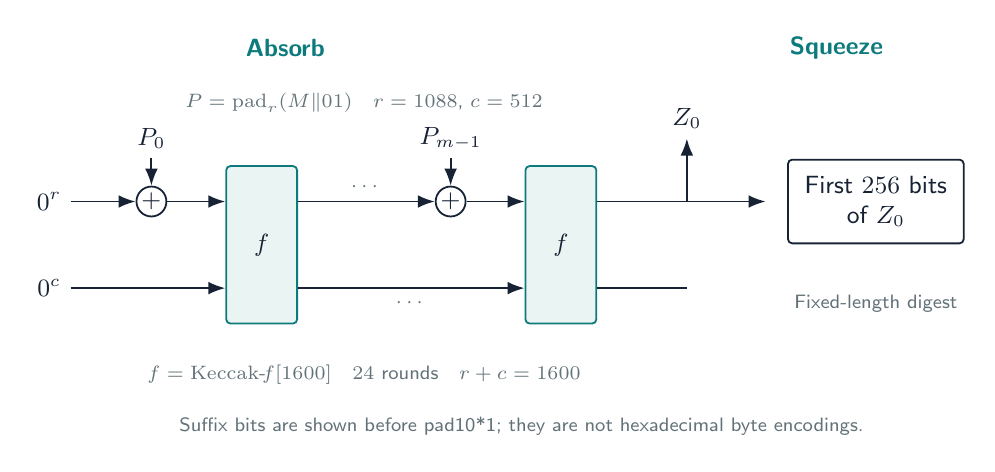
\begin{tikzpicture}
  \node[phase] at (3,2.25) {Absorb}; \node[phase] at (10,2.25) {Squeeze};
  \node[note] at (4,1.55) {$P=\operatorname{pad}_{r}(M\Vert\AtlasDomain)$\quad $r=\AtlasRate$, $c=\AtlasCapacity$};
  \node (zeroR) at (0,.3) {$0^r$}; \node (zeroC) at (0,-.8) {$0^c$};
  \node[xor] (x1) at (1.3,.3) {$+$}; \node[xor] (xn) at (5.1,.3) {$+$};
  \node[accent,minimum width=.9cm,minimum height=2cm] (f1) at (2.7,-.25) {$f$};
  \node[accent,minimum width=.9cm,minimum height=2cm] (fn) at (6.5,-.25) {$f$};
  \draw[wire] (zeroR) -- (x1); \draw[wire] (x1) -- (f1.west |- x1);
  \draw[wire] (zeroC) -- (f1.west |- zeroC);
  \draw[wire] (f1.east |- x1) -- node[above,note] {$\cdots$} (xn);
  \draw[wire] (xn) -- (fn.west |- xn);
  \draw[wire] (f1.east |- zeroC) -- node[below,note] {$\cdots$} (fn.west |- zeroC);
  \node at (1.3,1.1) {$P_0$}; \draw[wire] (1.3,.85) -- (x1);
  \node at (5.1,1.1) {$P_{m-1}$}; \draw[wire] (5.1,.85) -- (xn);
  \draw[wire] (fn.east |- xn) -- (8.1,.3) -- (8.1,1.1) node[above] {$Z_0$};
  \ifAtlasXof
    \node[accent,minimum width=.9cm,minimum height=2cm] (fout) at (10,-.25) {$f$};
    \draw[wire] (8.1,.3) -- (fout.west |- xn);
    \draw[wire] (fn.east |- zeroC) -- (fout.west |- zeroC);
    \draw[wire] (fout.east |- xn) -- (11.4,.3) -- (11.4,1.1) node[above] {$Z_1,\ldots$};
    \draw (fout.east |- zeroC) -- (11.4,-.8);
    \node[note] at (10,-1.8) {Return $d$ requested bits};
  \else
    \node[box] at (10.5,.3) {First $\AtlasOutputBits$ bits\\of $Z_0$};
    \draw[wire] (8.1,.3) -- (9.1,.3);
    \draw (fn.east |- zeroC) -- (8.1,-.8);
    \node[note] at (10.5,-1) {Fixed-length digest};
  \fi
  \node[note] at (4,-1.9) {$f=\kx$\quad $24$ rounds\quad $r+c=1600$};
  \node[note] at (6,-2.55) {Suffix bits are shown before pad10*1; they are not hexadecimal byte encodings.};
\end{tikzpicture}

\end{document}
